\section{Experiments and Results}


Detail exactly how you conducted the experiment so someone else could replicate it
\subsection{Setup}
\subsubsection{Dataset Generation}

\subsubsection{Benchmark}
Mention greedy baseline

\subsubsection{Hardware / Environment}

\subsection{Results}

\begin{itemize}
	\item Performance Metrics
	\item Plots
\end{itemize}

\begin{figure}[H]
	\begin{center}
		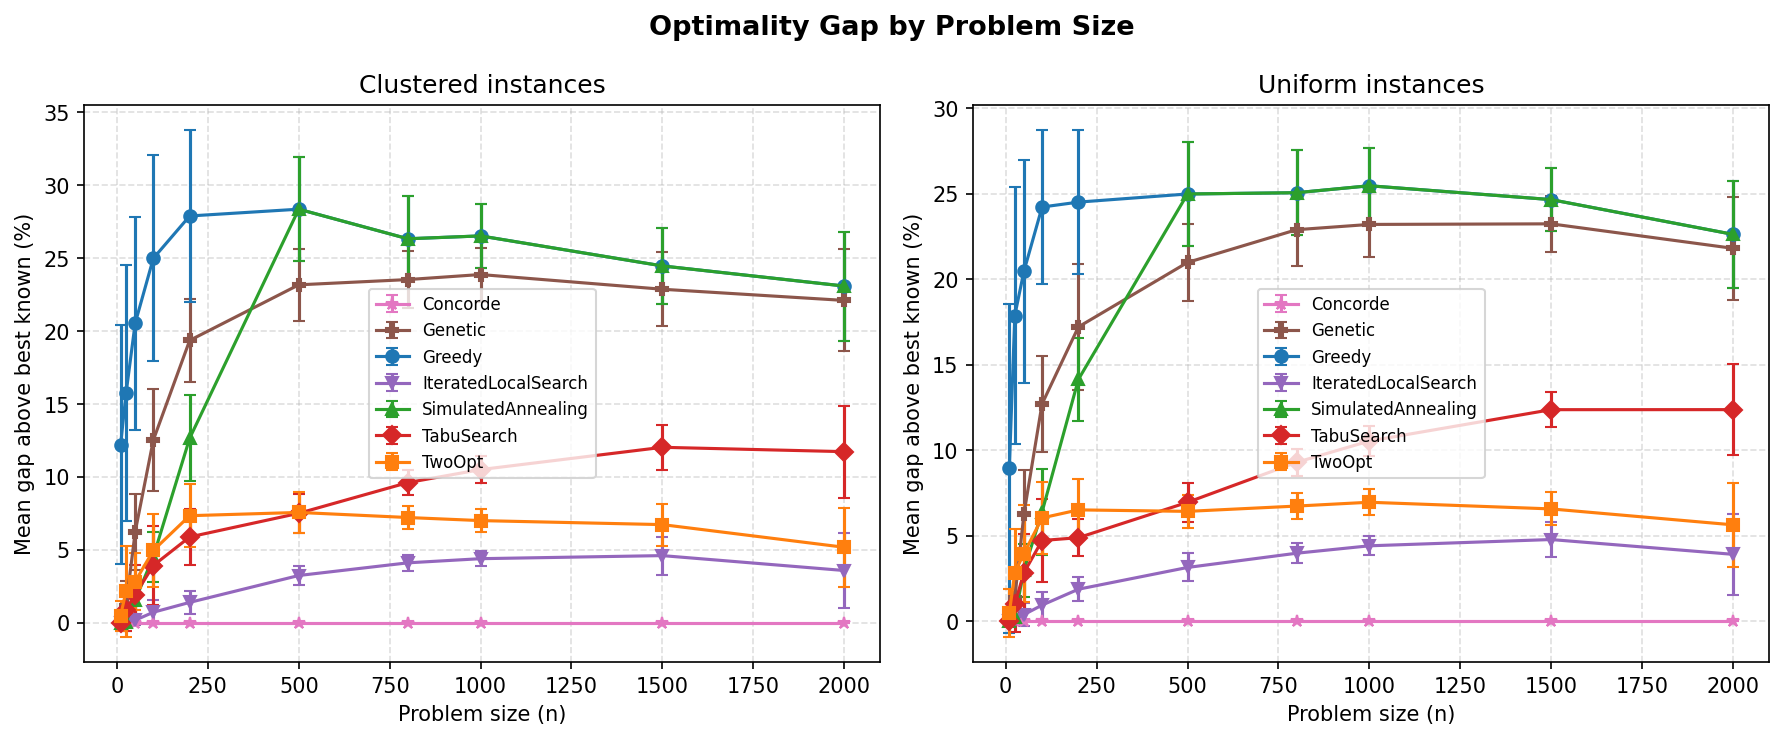
\includegraphics[width=0.95\linewidth]{figures/optimality_gap_lines.png}
	\end{center}
	\caption{Optimality gap of algorithms for different sizes and distributions}\label{fig:optimality_gap_lines}
\end{figure}

\textcolor{red}{Probably split Figure~\ref{fig:optimality_gap_lines} in half, so that it is nicely visible in single column layout.}

\begin{figure}[H]
	\begin{center}
		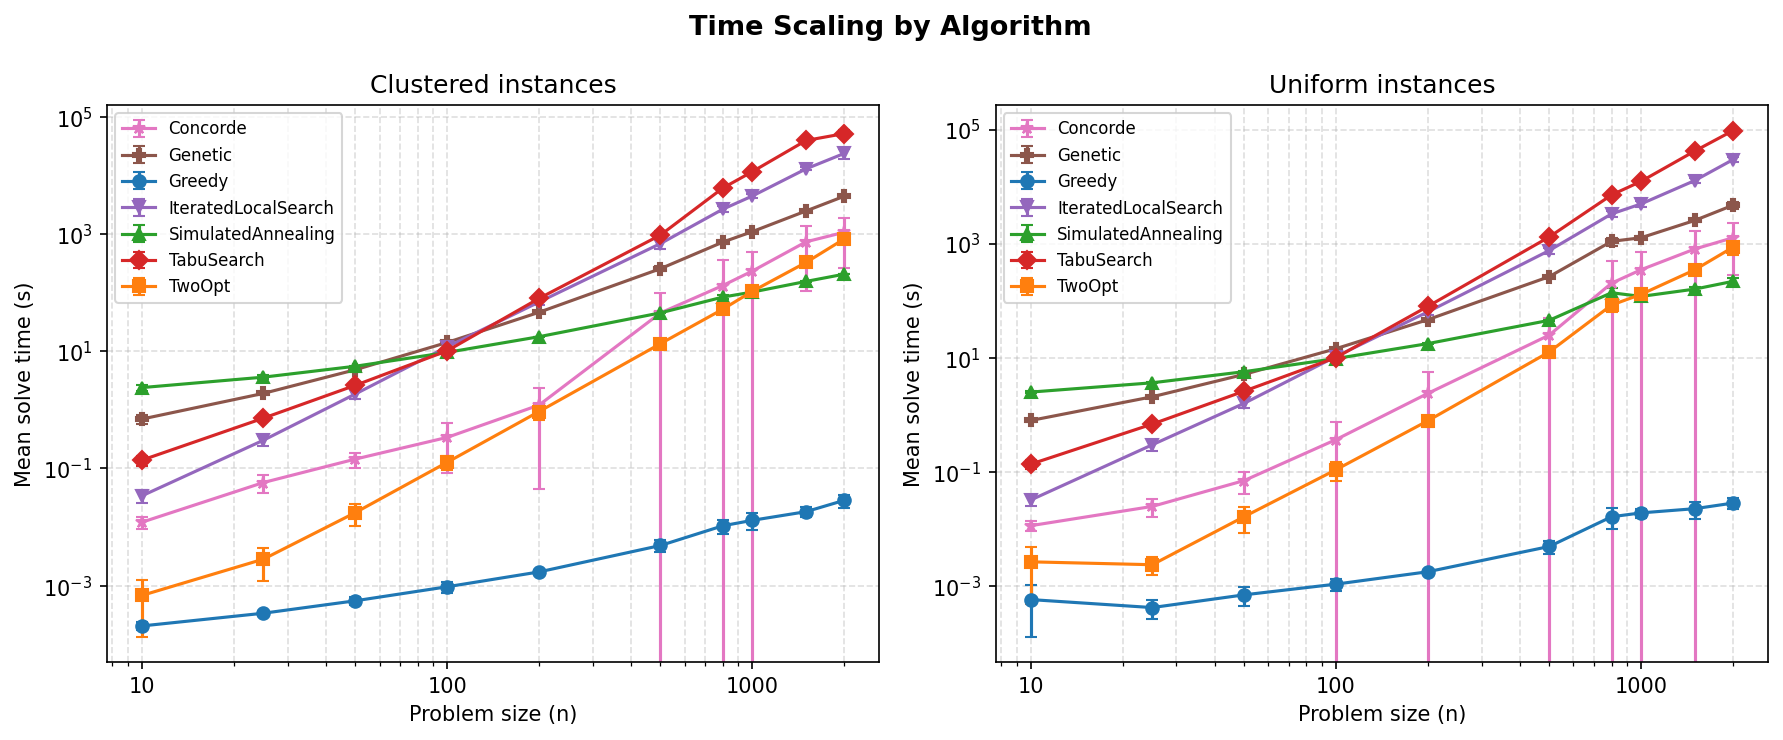
\includegraphics[width=0.95\linewidth]{figures/time_scaling.png}
	\end{center}
	\caption{Time scaling of algorithms for different sizes and distributions.}\label{fig:time_scaling}
\end{figure}

